
%%%%%%%%%%%%%%%%%%%%%%%%%%%%%%%%%%%%%%%%%%%%%%%%%%%%%%%%%%%%%%%%%%%%%
% LaTeX Template: Project Titlepage Modified (v 0.1) by rcx
%
% Original Source: http://www.howtotex.com
% Date: February 2014
% 
% This is a title page template which be used for articles & reports.
% 
% This is the modified version of the original Latex template from
% aforementioned website.
% 
%%%%%%%%%%%%%%%%%%%%%%%%%%%%%%%%%%%%%%%%%%%%%%%%%%%%%%%%%%%%%%%%%%%%%%

\documentclass[12pt]{article}
\usepackage[utf8]{inputenc}
\usepackage[a4paper]{geometry}
\usepackage[myheadings]{fullpage}
\usepackage{enumitem}
\usepackage{fancyhdr}
\usepackage{lastpage}
\usepackage{graphicx, wrapfig, subcaption, setspace, booktabs}
\usepackage[T1]{fontenc}
\usepackage[font=small, labelfont=bf]{caption}
\usepackage{fourier}
\usepackage{amsmath}
\usepackage[protrusion=true, expansion=true]{microtype}
\usepackage[english]{babel}
\usepackage{sectsty}
\usepackage{url, lipsum}
\usepackage{titlesec}
\usepackage{diagbox}
\usepackage{pdfpages}

\usepackage{listings}
\usepackage{color}

\definecolor{dkgreen}{rgb}{0,0.6,0}
\definecolor{gray}{rgb}{0.5,0.5,0.5}
\definecolor{mauve}{rgb}{0.58,0,0.82}

\lstset{frame=tb,
  language=C++,
  aboveskip=3mm,
  belowskip=3mm,
  showstringspaces=false,
  columns=flexible,
  basicstyle={\small\ttfamily},
  numbers=none,
  numberstyle=\tiny\color{gray},
  keywordstyle=\color{blue},
  commentstyle=\color{dkgreen},
  stringstyle=\color{mauve},
  breakatwhitespace=true,
  breaklines=true,
  tabsize=2
}

\newcommand{\HRule}[1]{\rule{\linewidth}{#1}}
\onehalfspacing
\setcounter{tocdepth}{5}
\setcounter{secnumdepth}{5}
\inputencoding{utf8}

\titleformat{\paragraph}
{\normalfont\normalsize\bfseries}{\theparagraph}{1em}{}
\titlespacing*{\paragraph}
{0pt}{3.25ex plus 1ex minus .2ex}{1.5ex plus .2ex}

%-------------------------------------------------------------------------------
% HEADER & FOOTER
%-------------------------------------------------------------------------------
\pagestyle{fancy}
\fancyhf{}
\setlength\headheight{15pt}
\fancyhead[L]{António Pedro Araújo Fraga}
\fancyhead[R]{Cranfield University}
\fancyfoot[R]{Page \thepage\ of \pageref{LastPage}}
%-------------------------------------------------------------------------------
% TITLE PAGE
%-------------------------------------------------------------------------------

\begin{document}

\title{ \fontsize{40}{90} \textsc{Computational Methods \& C++}
		\\ [2.0cm]
		\HRule{0.5pt} \\
		\LARGE \textbf{Heat Conduction Equation}
		\HRule{2pt} \\ [0.5cm]
		\normalsize \today \vspace*{5\baselineskip}}

\date{}

\author{
		\textbf{António Pedro Araújo Fraga} \\
		\textbf{Student ID: 279654} \\ 
		\textbf{Cranfield University} \\
		\textbf{M.Sc. in Software Engineering for Technical Computing
		} }

\maketitle
\thispagestyle{empty}
\newpage
\tableofcontents
\thispagestyle{empty}
\newpage
\null\vspace{\fill}
\begin{abstract}
\normalsize
Four numerical schemes were applied to compute a solution for a parabolic partial differential equation, the heat conduction equation. Two different types of schemes were used, explicit and implicit, and their solutions were evaluated. It could be observed the different behaviours of unstable and stable schemes. Step size variations of a stable method were studied as well. The obtained solutions were compared to the problem analytical solution in order to have a better understanding on these different behaviours.
\end{abstract}
\vspace{\fill}
\thispagestyle{empty}
\newpage

%-------------------------------------------------------------------------------
% Section title formatting
\sectionfont{\scshape}
\titleformat{\section}
{\normalfont\huge\bfseries}{\thesection}{1em}{}
\titleformat{\subsection}
{\normalfont\large\bfseries}{\thesubsection}{1em}{}
\titlespacing*{\section}
{0pt}{5.5ex plus 1ex minus .2ex}{4.3ex plus .2ex}
\titlespacing*{\subsection}
{0pt}{5.5ex plus 1ex minus .2ex}{4.3ex plus .2ex}
%-------------------------------------------------------------------------------

%-------------------------------------------------------------------------------
% BODY
%-------------------------------------------------------------------------------

%-------------------------------------------------------------------------------
% Nomenclature
%-------------------------------------------------------------------------------
\begin{table}[tb]
\caption{Nomenclature}
\label{tab:notation}
\centering
\def\arraystretch{1.5}
\begin{tabular}{ll}
Diffusivity & $D$\\
First derivative in time & $\frac{\partial f}{\partial t}$\\
First derivative in space & $\frac{\partial f}{\partial x}$\\
Time grid position & $n$\\
Space grid position & $i$\\
Function at time and space grid position & $f_i^n$\\
Time step & $\Delta t$\\
Space step & $\Delta x$\\
Time value & $t$\\
Space value & $x$\\
Analytical function at specific space and time values& $f(x, t)$\\
Initial Temperature& $T_{in}$\\
Surface Temperature& $T_{sur}$\\
\end{tabular}
\end{table}

%-------------------------------------------------------------------------------
% Introduction
%-------------------------------------------------------------------------------

\section*{Introduction}
\addcontentsline{toc}{section}{Introduction}
Numerical methods are used to obtain an approximated solution to problems with no given analytical solution. These methods can be used in order to save computational time, therefore they can obtain results which are similar to the real solution more efficiently. Four different schemes were applied to compute an approximated solution to a \textbf{Parabolic Partial Differential Equation}, in this case the heat conduction equation. 
\begin{center}
\Large
$
\frac{\partial f}{\partial t} = D\frac{\partial ^2 f}{\partial x^2} 
$
\end{center}
\par 
This condition had to be satisfied on a grid in space and time, which means the problem has a structured mesh type, and therefore can be represented as a grid of two dimensions. The previous equation could be written in its discretized form for each method.

\subsection*{Problem definition}
\addcontentsline{toc}{subsection}{Problem definition}
A few initial or boundary conditions were set, including the heat conduction equation. An existing wall with \textbf{1 \textit{ft}} thick had an initial temperature of \textbf{100ºF} and the surface temperatures at both sides were suddenly increased and maintained to \textbf{300ºF}. It is also known that the wall is composed of nickel steel (40\% Ni) with a Diffusivity of \textbf{0.01 $ft ^2/h$}.
\par
Since the wall has a 1 \textit{ft} thickness, the problem space domain could be restricted between \textbf{0} and \textbf{1}, and the diffusivity value, which is considered constant, could be set to \textbf{0.01}. The time domain was restricted between \textbf{0} to \textbf{0.5}:
\begin{center}
\normalsize
$
x \in [0, 1], t \in [0, 0.5]
$
\end{center}
\begin{center}
\normalsize
$
T_{in} = 100, T_{sur} = 300
$
\end{center}
\begin{center}
\normalsize
$
D = 0.01
$
\end{center}
\par 
The initial boundaries can be formalized in mathematical expressions:
\begin{center}
\normalsize
$
f(x,0) = T_{in}
$
\end{center}
\begin{center}
\normalsize
$
f(0,t) = T_{sur}
$
\end{center}
\begin{center}
\normalsize
$
f(1,t) = T_{sur}
$
\end{center}
\par
The analytical solution of this problem was given by the following expression:
\begin{center}
\normalsize
$$
f(x,t) = T_{sur} + 2(T_{in} - T_{sur}) \sum_{m=1}^{m=\infty} 
e ^{-D t (m \pi / L) ^2}  \frac{1 - (-1)^m}{m \pi} sin \left(\frac{m \pi x}{L}\right)$$  

\end{center}

\subsection*{Numerical analysis}
\addcontentsline{toc}{subsection}{Numerical analysis}
\par Numerical analysis is the study of the obtained solution. Criticism is very important on this phase, since the solutions are evaluated. Digital computers have problems with round-off errors, and since values were truncated, problems with discretization errors may appear. There are some definitions related with this study: stability, convergence and approximation \cite{convergence_stability_consistency, numerical_analysis}.

\par A method is declared stable if the error doesn't grow as time advances. Theoretically, conditions that make a scheme becomes stable or unstable can be known.
\par Approximation can be verified by comparing the computed solution with the analytical solution, and check if there is an approximation at all.
\par Convergence is defined by how well the computed solution approximates to the analytical solution. This can vary with a change in the number of \textbf{time steps} or \textbf{space steps}. A smaller number of steps can lead to a bigger error, whereas a bigger number of steps can lead to a considerably more time expensive solution. Every method could be developed using \textbf{Taylor Series} \cite{hoffman}. This series were developed for \textbf{n} terms. Thus, every method has a given approximation factor, that could be represented in the \textbf{Big Oh} annotation. The error related with this approximation is called \textbf{Truncation Error} \cite{numerical_analysis}.
\par A quantitative analysis can be done by comparing solutions of each method. By calculating the \textbf{norms} of the error matrix, one can conclude which method is more accurate. The \textbf{error matrix} can be calculated by subtracting each cell of the \textbf{analytical} solution matrix to the cells of a method matrix. When the result is a matrix of small values, the error is small. Whenever a norm is calculated, one is able to translate an error matrix into a single value:

\begin{itemize}[noitemsep] 
\item \textbf{One Norm} - Which is given by adding the absolute values of each cell of the matrix.
\item \textbf{Two Norm} - Which is obtained by adding the squares of every value in the matrix.
\item \textbf{Uniform Norm} - Which represents the biggest error, or the maximum value in the matrix.
\end{itemize}

The second norm "punishes" the biggest values, and "regards" the lowest ones. Notice that a the square of a value between $0$ and $1$ is lower than the given value. Whereas the square of a value bigger than 1 is higher. Therefore, this norm is a good quality indicator. 

\par A stencil could also be developed for each method, which relates the several grid points, revealing the dependencies for a calculation in a more graphical way. 

\section*{Procedures}
\addcontentsline{toc}{section}{Procedures}
Four different schemes/methods were used to compute a solution for the given problem, two of them are explicit schemes, \textbf{Richardson}, \textbf{DuFort-Frankel}, and two of them are implicit schemes, \textbf{Laasonen Simple Implicit} and \textbf{Crank-Nicholson}. The space step was maintained at \textbf{0.05} \textit{ft}, and the time step took the value of \textbf{0.01} \textit{h}, studying every solutions in intervals of \textbf{0.1} hours from \textbf{0.0} to \textbf{0.5}. The \textbf{Laasonen Simple Implicit} solution was also studied with different time steps, always maintaining the same space step,  \textbf{$\Delta x = 0.05$}:
\begin{itemize}[noitemsep] 
\item $ \Delta t = 0.01 $
\item $ \Delta t = 0.025 $
\item $ \Delta t = 0.05 $
\item $ \Delta t = 0.1 $
\end{itemize}
As referred, considering the initial equation, these methods can be written in its discretized form.

\subsection*{Explicit Schemes}
\addcontentsline{toc}{subsection}{Explicit Schemes}

\par This type of schemes rely only on the previous time steps to calculate the current time step solution. In the case of both used methods, they were relying in known values of the \textbf{n - 1} and \textbf{n} time steps to calculate a value for the \textbf{n + 1} time step. Thereby, the second time step can not be calculated by these methods, because there's no possible value for a negative time step. A different method, for the same equation, with two levels of time steps was used in order to overcome this situation, the \textbf{Forward in Time and Central in Space} scheme. It's known that this method is \textbf{conditionally stable}, and its stability condition is given by\cite{hoffman},

\begin{center}
\Large
$
\frac{D \Delta t}{(\Delta x)^2} \leq 0.5
$
\end{center}

Therefore, considering $\Delta t = 0.01$, $\Delta x = 0.05$, and $D = 0.1$, this method is declared stable. It's important to have a stable solution for the first iteration, since it is a major influence on the overall solution\cite{heat_transfer}. Therefore, this iteration could be calculated with the following expression,

\begin{center}
\Large
$
f_{i}^{n + 1} = f_{i}^{n} + \frac{D \Delta t}{(\Delta x)^2}(f_{i + 1}^{n} - 2f_{i}^{n} + f_{i - 1}^{n})
$
\end{center}

\begin{figure}[!htb]
\centering
\begin{minipage}{.5\textwidth}
  \centering
  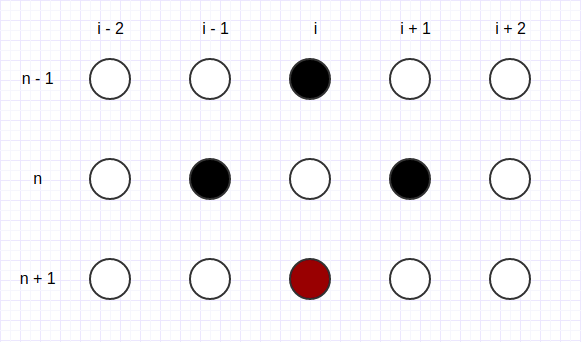
\includegraphics[width=.8\linewidth]{richardson.png}
  \captionof{figure}{DuFort-Frankel's method stencil.}
\end{minipage}%
\begin{minipage}{.5\textwidth}
  \centering
  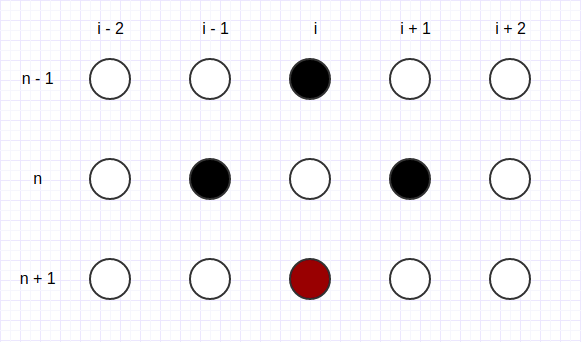
\includegraphics[width=.8\linewidth]{dufort-frankel.png}
  \captionof{figure}{Richardson's method stencil.}
\end{minipage}
\end{figure}

\subsubsection*{Richardson}
\addcontentsline{toc}{subsubsection}{Richardson}
The Richardson method can be applied by having a central in time and central in space scheme. Regarding to stability issues, this method is unconditionally unstable. This method is of order \textbf{O($\Delta x ^2$, $\Delta t ^2$)} \cite{hoffman}. Following the heat conduction equation, the expression could be represented at \textbf{Figure 2} and could be written as following:
\begin{center}
\Large
$
\frac{f_i^{n + 1} - f_i^{n - 1}}{2 \Delta t} = D \frac{f_{i + 1}^{n} - 2f_{i}^{n} + f_{i - 1}^{n}}{(\Delta x)^2}
$
\end{center}
\par Which corresponds to,
\begin{center}
\Large
$
f_{i}^{n + 1} = f_{i}^{n - 1} - \frac{2\Delta t D}{(\Delta x)^2} (f_{i + 1}^{n} - 2 f_{i}^{n} + f_{i - 1}^{n})
$
\end{center}

\subsubsection*{DuFort-Frankel}
\addcontentsline{toc}{subsubsection}{DuFort-Frankel}
\par The DuFort-Frankel scheme can be applied by having central differences in both derivatives, but to prevent stability issues, the space derivative term $f_i^n$ can be written as the average value of $f_{i}^{n + 1}$ and $f_{i}^{n - 1}$. The method stencil can be observed at \textbf{Figure 1}. Therefore this method is of order \textbf{O($\Delta x ^2$, $\Delta t ^2$, $(\frac{\Delta t}{\Delta x}) ^2$)} \cite{hoffman}, it is declared as unconditionally stable and it may be formulated as follows:
\begin{center}
\Large
$
\frac{f_i^{n + 1} - f_i^{n - 1}}{2 \Delta t} = D \frac{f_{i + 1}^{n} - f_{i}^{n + 1} - f_{i}^{n - 1} + f_{i - 1}^{n}}{(\Delta x)^2}
$
\end{center}
\par Which is equivalent to,
\begin{center}
\Large
$
f_{i}^{n + 1} = f_{i}^{n - 1} - \frac{2\Delta t D}{(\Delta x)^2} (f_{i + 1}^{n} - f_{i}^{n + 1} - f_{i}^{n - 1} + f_{i - 1}^{n})
$
\end{center}

\subsection*{Implicit Schemes}
\addcontentsline{toc}{subsection}{Implicit Schemes}

\par In other hand, implicit schemes rely not only on lower time steps to calculate a solution, but also on the current time step known values. Each time step solution can often be solved by applying the Thomas Algorithm, which is an algorithm that can solve tridiagonal matrix systems, $Ax = r$\cite{thomas}. This algorithm is a special case of the LU decomposition, with a better performance. The matrix $A$ can be decomposed in a lower triangular matrix $L$ and an upper triangular matrix $U$, therefore $A = LU$\cite{thomas}. This algorithm consists of two steps, the downwards phase where the equation $Lp = r$ is solved and the upwards phase, solving $Ux = p$\cite{thomas}, obtaining a solution for $x$. 

\begin{figure}[!htb]
\centering
\begin{minipage}{.5\textwidth}
  \centering
  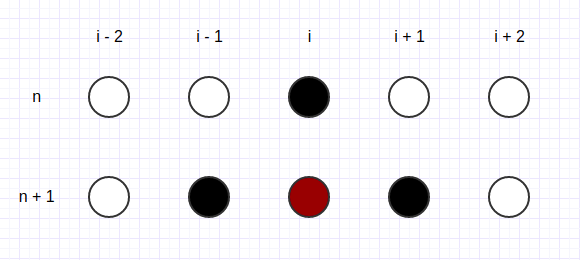
\includegraphics[width=.8\linewidth]{laasonen.png}
  \captionof{figure}{Laasonen's method stencil.}
\end{minipage}%
\begin{minipage}{.5\textwidth}
  \centering
  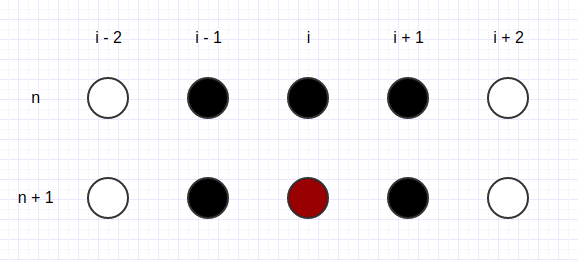
\includegraphics[width=.8\linewidth]{crank-nicholson.png}
  \captionof{figure}{Crank-Nicholson's method stencil.}
\end{minipage}
\end{figure}

\subsubsection*{Laasonen Simple Implicit}
\addcontentsline{toc}{subsubsection}{Laasonen Simple Implicit}
\par The time derivative is considered forward in time. Central difference is used in space derivative, and the scheme is of order \textbf{O($\Delta x $, $\Delta t ^2$)}\cite{hoffman}, and unconditionally stable. Concluding, the below equation could be established, and it could be represented at \textbf{Figure 3}:

\begin{center}
\Large
$
\frac{f_i^{n + 1} - f_i^{n}}{\Delta t} = D \frac{f_{i + 1}^{n + 1} - 2f_{i}^{n + 1} + f_{i - 1}^{n + 1}}{(\Delta x)^2} 
$
\end{center}

\par Assuming that $c = \frac{\Delta t D}{(\Delta x)^2}$, the equation could be represented as:

\begin{center}
\Large
$
(1 - 2c)f_i^{n + 1} = f_i^n + c \left[f_{i + 1}^{n + 1} + f_{i - 1}^{n + 1}\right]
$
\end{center}

\par The values of the first and last space position of each time step are known, they are represent by the $T_{sur}$ value. Therefore, in every second and penultimate space step, two terms of the previous equation could be successfully inquired. For the second space step, the equation could be divided by having the unknown terms in the left side and the known terms in the right side:

\begin{center}
\Large
$
(1 - 2c)f_i^{n + 1} - c f_{i + 1}^{n + 1} = f_i^n + c f_{i - 1}^{n + 1}
$
\end{center}

\par And the same could be done for the penultimate space step:

\begin{center}
\Large
$
(1 - 2c)f_i^{n + 1} - c f_{i - 1}^{n + 1} = f_i^n + c f_{i + 1}^{n + 1}
$
\end{center}

\par For every other space steps with unknown values, the expression could be generalized as:

\begin{center}
\Large
$
(1 - 2c)f_i^{n + 1} - c \left[f_{i + 1}^{n + 1} + f_{i - 1}^{n + 1}\right] = f_i^n 
$
\end{center}

\par Considering that the maximum number of space steps is \textbf{m}, the previous expressions could form a system of linear equations, $A.x = r$:
\begin{center}
$
\begin{bmatrix}
    (1 - 2c) & -c & 0 & 0 & \dots & 0 & 0 \\
    -c & (1 - 2c) & -c & 0 & \dots & 0 & 0 \\
    0 & -c & (1 - 2c) & -c & \dots & 0 & 0 \\
    \hdotsfor{7} \\
    0 & 0 & 0 & 0 & \dots & -c & (1 - 2c) \\
\end{bmatrix}
\begin{bmatrix}
    f_1^{n + 1} \\
    f_2^{n + 1} \\
    f_3^{n + 1} \\
    \dots \\
    f_{\textbf{m} - 1}^{n + 1} \\
\end{bmatrix}
=
\begin{bmatrix}
    f_1^{n} + c f_0^{n + 1} \\
    f_2^{n} \\
    f_3^{n} \\
    \dots \\
    f_{\textbf{m} - 1}^{n} + c f_{\textbf{m}}^{n + 1} \\
\end{bmatrix}
$
\end{center}


\subsubsection*{Crank-Nicholson}
\addcontentsline{toc}{subsubsection}{Crank-Nicholson}
\par The time derivative is considered forward in time, and the space derivative can be replaced by the average of central differences in time steps \textbf{n} and \textbf{n + 1}. The method is of order \textbf{O($\Delta x ^2$, $\Delta t ^2$)} \cite{hoffman}, is declared unconditionally stable and it could be represented at \textbf{Figure 4}. Thus:

\begin{center}
\Large
$
\frac{f_i^{n + 1} - f_i^{n}}{\Delta t} = \frac{1}{2} D {\left[\frac{f_{i + 1}^{n + 1} - 2f_{i}^{n + 1} + f_{i - 1}^{n + 1}}{(\Delta x)^2} + \frac{f_{i + 1}^{n} - 2f_{i}^{n} + f_{i - 1}^{n}}{(\Delta x)^2}\right]}
$
\end{center}

\par In this method, the coefficient had a new value, $c = \frac{1}{2}\frac{\Delta t D}{(\Delta x)^2}$, and assuming that $p = f_{i + 1}^{n} + f_{i - 1}^{n}$, the equation could be written as follows,

\begin{center}
\Large
$
(1 - 2c)f_i^{n + 1} = (1 - 2c)f_i^n + c \left[f_{i + 1}^{n + 1} + f_{i - 1}^{n + 1} + p\right]
$
\end{center}

\par Following the same logical principles of the previous scheme, 
some expressions could be generalized for the second,

\begin{center}
\Large
$
(1 - 2c)f_i^{n + 1} - c f_{i + 1}^{n + 1} = (1 - 2c)f_i^n + c \left[f_{i - 1}^{n + 1} + p\right]
$
\end{center}
, penultimate, 
\begin{center}
\Large
$
(1 - 2c)f_i^{n + 1} - c f_{i + 1}^{n + 1} = (1 - 2c)f_i^n + c \left[f_{i + 1}^{n + 1} + p\right]
$
\end{center}
, and every other space steps with unknown values.

\begin{center}
\Large
$
(1 - 2c)f_i^{n + 1} - c \left[f_{i + 1}^{n + 1} + f_{i - 1}^{n + 1}\right] = (1 - 2c)f_i^n + cp
$
\end{center}

\par Thus, a tridiagonal matrix system is obtained,

\begin{center}
\small
$
\begin{bmatrix}
    (1 - 2c) & -c & 0 & 0 & \dots & 0 & 0 \\
    -c & (1 - 2c) & -c & 0 & \dots & 0 & 0 \\
    0 & -c & (1 - 2c) & -c & \dots & 0 & 0 \\
    \hdotsfor{7} \\
    0 & 0 & 0 & 0 & \dots & -c & (1 - 2c) \\
\end{bmatrix}
\begin{bmatrix}
    f_1^{n + 1} \\
    f_2^{n + 1} \\
    f_3^{n + 1} \\
    \dots \\
    f_{\textbf{m} - 1}^{n + 1} \\
\end{bmatrix}
=
\begin{bmatrix}
    (1 - 2c)f_1^{n} + c \left[f_0^{n + 1} + p\right] \\
    (1 - 2c)f_2^{n} + cp \\
    (1 - 2c)f_3^{n} + cp\\
    \dots \\
    (1 - 2c)f_{\textbf{m} - 1}^{n} + c \left[f_{\textbf{m}}^{n + 1} + p\right] \\
\end{bmatrix}
$
\end{center}

\section*{Solution Design}
\addcontentsline{toc}{section}{Solution Design}
\par The code was first planned with an initial structure and suffered incremental upgrades. A \textbf{method} class was created, being a prototype with multiple inheritance, containing three sub classes: \textbf{Analytical}, \textbf{Implicit} and \textbf{Explicit}. Therefore, the \textbf{Implicit} class is an Abstract class as well. This class has three sub classes, representing the three explicit methods used in this problem. Similarly, the \textbf{Implicit} class is also an abstract class, having two implicit methods classes as sub classes. The previously described inheritance structure can be more easily visualized on \textbf{Figure 5}.

\begin{figure}[!htb]
  \centering
  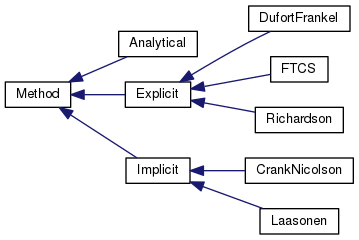
\includegraphics[width=.5\linewidth]{method_inheritance.png}
  \captionof{figure}{Method Class inheritance diagram.}
\end{figure}

\par A Method class contains a \textbf{Problem} object. The \textbf{Problem} class represents the Heat Conduction problem, containing informations about the time and space steps, the solution and initial conditions.
\par An \textbf{Input and Output Manager} class was developed so that the code related with plots and tables exportations could be separated from the logical source code. This class was developed with several methods regarding data interpretation and structuration in order to easily export plot charts. A \textbf{gnuplot c++ library} was used, therefore the gnuplot syntax could be directly used from the c++ code, cutting down the need of developing external bash scripts for this specific purpose.
\par Despite the referred classes, a header file with useful \textbf{macros} was declared. This file contains information about which conditions to test, like the initial temperature and the surface temperature. Therefore, if for some reason, one of this values changes, it can be easily corrected.
\par The \textbf{Matrix} and \textbf{Vector} classes, which were provided in the c++ module were reused to represent a solution matrix or a solution vector of a certain iteration.
\par The several objects in this structure could be instantiated in the main file, calling methods to compute the several solutions and to export their plot charts. The previously described classes can be represented in the \textbf{Figure 6} diagram.

\begin{figure}[!htb]
  \centering
  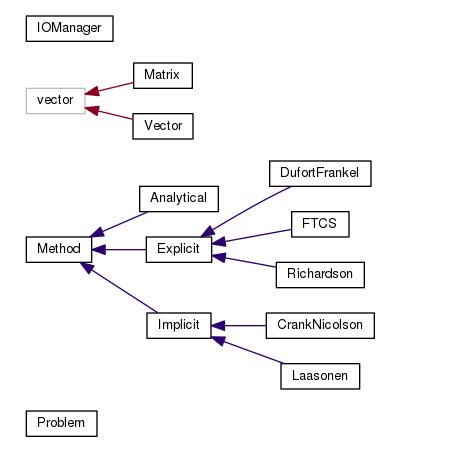
\includegraphics[width=.5\linewidth]{class_diagram.png}
  \captionof{figure}{Class Diagram.}
\end{figure} 

\section*{Results \& Discussion}
\addcontentsline{toc}{section}{Results \& Discussion}
\par The results of the four methods, \textbf{Richardson}, \textbf{DuFort-Frankel}, \textbf{Laasonen Simple Implicit} and \textbf{Crank-Nicholson} can be seen in the following figures/tables. These results were used to analyze each solution quantitatively and qualitatively. In most of the plot charts, the obtained solution was compared to the analytical solution so that it would be possible to realize whether the solution was a good approximation or not. Notice that the next results are regarding to the "default" values of time and space steps, $\Delta t = 0.01$ and $\Delta x = 0.05$. 

\begin{table}[!htb]
\centering
\caption{Richardson method error table.}
\label{table:1}
\fontsize{6.5}{18}\selectfont
\begin{tabular}{|| c || c | c | c | c | c | c | c | c | c | c | c ||} 
 \hline
 \diagbox[width=5em]{t}{x} & 0.10 & 0.20 & 0.30 & 0.40 & 0.50 & 0.60 & 0.70 & 0.80 & 0.90 \\ [0.5ex] 
 \hline\hline
 0.1 & 1.05136e+06 & 631856 & 123707 & 8417.73 & 300.81 & 8417.73 & 123707 & 631856 & 1.05136e+06 \\ 
 0.2 & 1.33245e+11 & 1.39e+11 & 7.02854e+10 & 2.06123e+10 & 6.93136e+09 & 2.06123e+10 & 7.02854e+10 & 1.39e+11 & 1.33245e+11 \\
 0.3 & 2.14659e+16 & 2.74969e+16 & 1.97012e+16 & 9.88337e+15 & 5.98161e+15 & 9.88337e+15 & 1.97012e+16 & 2.74969e+16 & 2.14659e+16  \\
 0.4 & 3.91917e+21 & 5.60267e+21 & 4.87086e+21 & 3.31281e+21 & 2.58429e+21 & 3.31281e+21 & 4.87086e+21 & 5.60267e+21 & 3.91917e+21 \\ 
 0.5 & 7.74272e+26 & 1.19047e+27 & 1.18021e+27 & 9.72231e+26 & 8.60626e+26 & 9.72231e+26 & 1.18021e+27 & 1.19047e+27 & 7.74272e+26  \\[1ex] 
 \hline
\end{tabular}
\end{table}

\par By examining \textbf{Table 2}, it could be concluded that the solution given by the Richardson method  was considerably different from the analytical solution. This was due to the fact that this method is declared as \textbf{unconditionally unstable}.  As referred before, when a method is declared unstable, the error grows as the time advances. The error growth was responsible for obtaining a different solution, or a solution to a different problem. The mathematical calculations regarding the stability and accuracy properties of this method can be found under the appendix section. 

\begin{figure}[!htb]
  \centering
  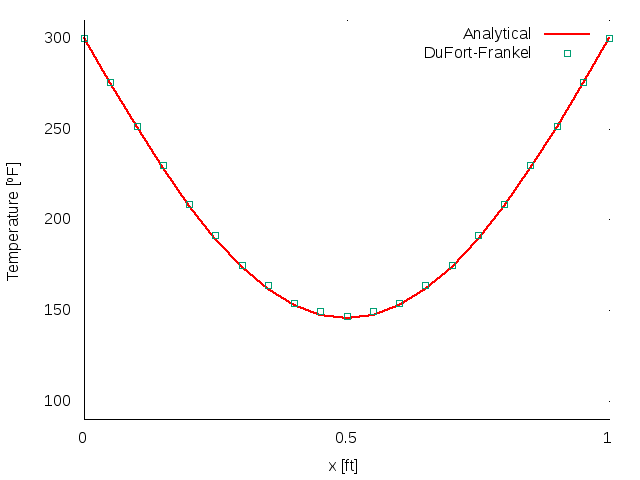
\includegraphics[width=.5\linewidth]{DuFort-Frankelt_0_5.png}
  \captionof{figure}{DuFort-Frankel's solution at $t= 0.5$.}
\end{figure}

\par When looking at \textbf{Figure 7}, it can be observed that the DuFort-Frankel solution is quite approximated to the real solution. This scheme, as it could be observed at \textbf{Figure 11}, is more time efficient comparing to the implicit unconditionally stable methods, the only disadvantage is the fact that it requires a different method for the first iteration.

\par Similarly of what could be concluded on DuFort-Frankel results, by observing \textbf{Figure 9} and \textbf{Figure 8}, it can also be deducted that these are good solutions. These schemes, Crank-Nicholson and Laasonen, are unconditionally stable as well. Therefore good results were expected.

\begin{figure}[!htb]
\centering
\begin{minipage}{.5\textwidth}
  \centering
  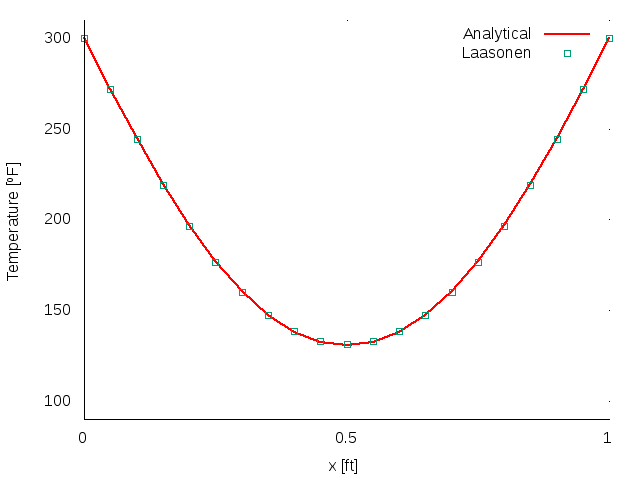
\includegraphics[width=.8\linewidth]{Laasonent_0_4dt_0_010.png}
  \captionof{figure}{Laasonen's solution at $t= 0.4$.}
\end{minipage}%
\begin{minipage}{.5\textwidth}
  \centering
  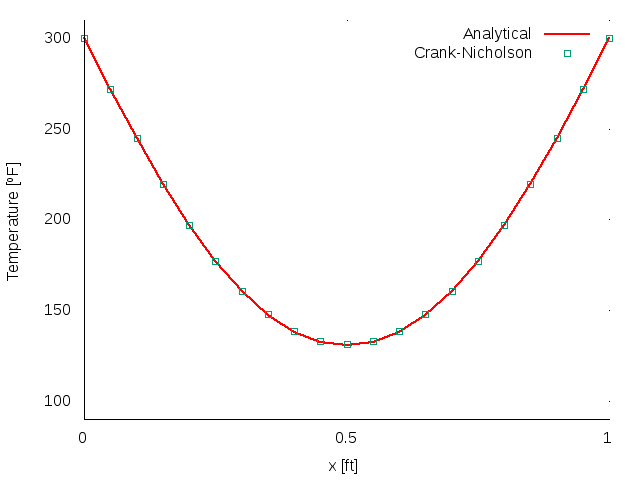
\includegraphics[width=.8\linewidth]{Crank-Nicholsont_0_4.png}
  \captionof{figure}{Crank-Nicholson's solution at $t= 0.4$.}
\end{minipage}
\end{figure}

\par In other hand, when a quantitative analysis was done, it could be seen that the Crank Nicholson scheme is more accurate than the Laasonen and DuFort-Frankel methods. By looking at \textbf{Figure 10}, it can be observed that the second norm value of the \textbf{Error matrix} of this scheme is smaller than the values obtained by the other methods \textbf{Error Matrices}.

\begin{figure}[!htb]
\centering
\begin{minipage}{.5\textwidth}
  \centering
  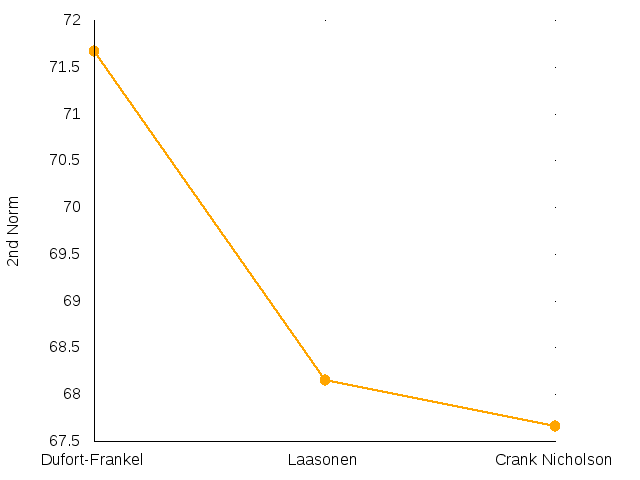
\includegraphics[width=.8\linewidth]{norms.png}
  \captionof{figure}{2nd norm values of Error Matrices.}
\end{minipage}%
\begin{minipage}{.5\textwidth}
  \centering
  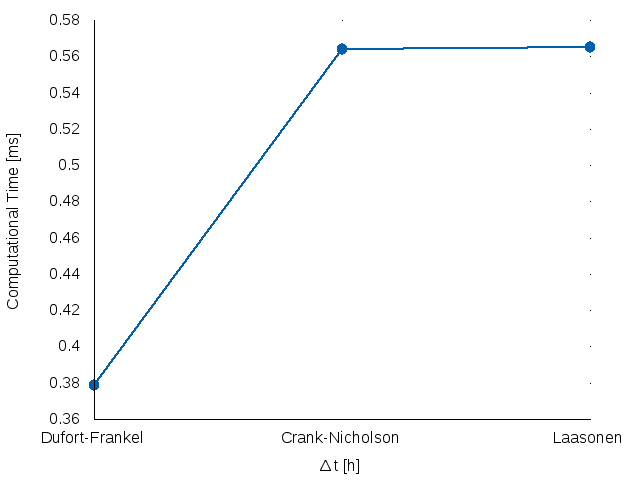
\includegraphics[width=.8\linewidth]{default_deltat_times.png}
  \captionof{figure}{Computational times of stable methods.}
\end{minipage}
\end{figure}

\subsection*{Laasonen Implicit Scheme: study of time step variation}
\addcontentsline{toc}{subsection}{Laasonen Implicit Scheme: study of time step variation}

\par Laasonen Implicit Scheme is an unconditionally stable scheme to solve Parabolic Partial Differential Equations. Therefore, with the right time and space step, there's almost no error related to the development of its results throughout the time advancement. 
\par A reduction on these steps led to a higher computational time, since there's more calculations to be made. Whereas steps with higher values led to more inaccurate results\cite{step_size}. This phenomenon could be explained with a concept that was introduced earlier, the \textbf{truncation error}\cite{hoffman}. This error can only be avoided with exact calculations, but can be reduced by applying a larger number of smaller intervals or steps. As referred before, different results of this method were studied by changing the time step size. The space step was maintained, $\Delta x = 0.05$.

\begin{table}[!htb]
\centering
\caption{Laasonen method error table for the several $\Delta t$ at $t = 0.5$}
\label{table:1}
\fontsize{8}{18}\selectfont
\begin{tabular}{|| c || c | c | c | c | c | c | c | c | c | c | c ||} 
 \hline
 \diagbox[width=5em]{$\Delta t$}{x} & 0.10 & 0.20 & 0.30 & 0.40 & 0.50 & 0.60 & 0.70 & 0.80 & 0.90 \\ [0.5ex] 
 \hline\hline
 0.01 & 0.288694 & 0.385764 & 0.255427 & 0.0405061 & -0.0611721 & 0.0405061 & 0.255427 & 0.385764 & 0.288694 \\ 
 0.025 & 0.738044 & 1.0344 & 0.805442 & 0.368491 & 0.157551 & 0.368491 & 0.805442 & 1.0344 & 0.738044 \\
 0.05 & 1.53627 & 2.15669 & 1.71375 & 0.864487 & 0.457364 & 0.864487 & 1.71375 & 2.15669 & 1.53627  \\
 0.1 & 3.29955 & 4.49523 & 3.46045 & 1.7082 & 0.898726 & 1.7082 & 3.46045 & 4.49523 & 3.29955 \\ [1ex] 
 \hline
\end{tabular}
\end{table}

\par \textbf{Table 3} and \textbf{figure 12} could support the previous affirmations.  While observing \textbf{table 3}, it could be seen that the error is larger for bigger time steps, as it was expected. Whereas when observing \textbf{figure 12}, it can be identified a reduction in computational time as the \textbf{time step} becomes larger.

\begin{figure}[!htb]
  \centering
  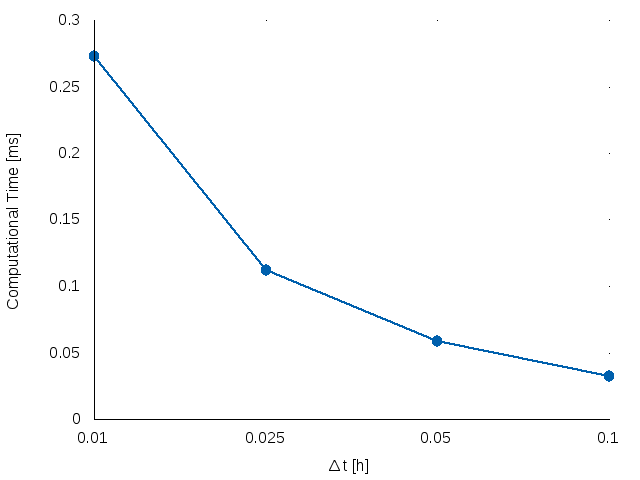
\includegraphics[width=.6\linewidth]{laasonen_times.png}
  \captionof{figure}{Laasonen method computational times for the several $\Delta t$.}
\end{figure}

\pagebreak
\section*{Conclusions}
\addcontentsline{toc}{section}{Conclusions}

\par The obtained results could support the theoretical concepts. Unstable methods demonstrated an error growth through the time progress. The \textbf{Forward in Time, Central in Space} explicit scheme was stable with the given initial conditions, therefore it could support a good solution for the explicit stable scheme, \textbf{DuFort-Frankel}. As referred, the solution of the DuFort-Frankel method strongly depends on the first iteration solution.
\par It could be observed that smaller steps can lead to a time expensive solution, whereas larger steps lead to an error increase. Stable methods could give a good solution with the right time and space steps, but by analysing the second norm value, it was concluded that the Crank-Nicholson method is more accurate. This is due to the fact that this method has a better approximation order.
\par It is important to have a balance between the two problems (time and approximation), a method should be computed in an acceptable time, and still obtain a good result. In realistic scenarios the problem solution is not known, therefore error estimates are impractical. The used step size should be small as possible, as long as the solution is not dominated with round-off errors. The solution must be obtained with a number of steps that one has time to compute. 
 

%-------------------------------------------------------------------------------
% REFERENCES
%-------------------------------------------------------------------------------
\newpage
%\addcontentsline{toc}{section}{References}
\begin{thebibliography}{0}

\bibitem{convergence_stability_consistency}
Gilberto E. Urroz, July 2004, \textit{Convergence, Stability, and Consistency of Finite
Difference Schemes in the Solution of Partial Differential
Equations,} Available at: <\url{http://ocw.usu.edu/Civil_and_Environmental_Engineering/Numerical_Methods_in_Civil_Engineering/StabilityNumericalSchemes.pdf}> [Accessed 2 October 2017]

\bibitem{numerical_analysis}
S. Scott Collis, April 26, 2005, \textit{An Introduction to Numerical Analysis
for Computational Fluid Mechanics,} [Accessed 2 October 2017]

\bibitem{hoffman}
Klaus A. Hoffman, Steve T. Chiang, August 2000, \textit{Computational Fluid Dynamics, Volume 1} [Accessed 27 October 2017]

\bibitem{heat_transfer}
Richard H. Pletcher, Jhon C. Tannehill, Dale A. Anderson, 2013, \textit{Computational Fluid Mechanics and Heat Transfer, Third Edition}, [Accessed 27 October 2017]

\bibitem{thomas}
W. T. Lee, \textit{Tridiagonal Matrices: Thomas Algorithm}, Available at: <\url{https://www3.ul.ie/wlee/ms6021_thomas.pdf}> [Accessed 28 October 2017]

\bibitem{error}
\textit{ Error in Euler’s Method}, Available at: <\url{http://www.math.unl.edu/~gledder1/Math447/EulerError}> [Accessed 2 November 2017]

\bibitem{step_size}
John D. Cook, February 22 2008, \textit{ Step size for numerical differential equations}, Available at: <\url{https://www.johndcook.com/NumericalODEStepSize.pdf}> [Accessed 3 November 2017]

\bibitem{explicit_implicit}
B.J.P. Kaus, \textit{Explicit versus implicit Finite Difference Schemes}, Available at: <\url{https://www.geowiss.uni-mainz.de/Dateien/Finite_Differerence_Timpl_expl.pdf}> [Accessed 4 November 2017]

\bibitem{numerical_methods_pde}
Markus Schmuck, \textit{Numerical Methods for PDEs}, Available at: <\url{http://www.macs.hw.ac.uk/~ms713/lecture_9.pdf}> [Accessed 10 November 2017]

\end{thebibliography}
\newpage

\section*{Appendices}
\addcontentsline{toc}{section}{Appendices}

\subsection*{Richardson Method Analysis}
\addcontentsline{toc}{subsection}{Richardson Method Analysis}

\subsubsection*{Accuracy}
\addcontentsline{toc}{subsubsection}{Accuracy}

Every term can be developed with Taylor expansions:


\begin{center}
\Large
$
f(x + \Delta t) = f_i^{n} + \Delta t \left( \frac{\partial f}{\partial t} \right)_i^n + \frac{\Delta t ^2}{2} \left( \frac{\partial ^2 f}{\partial t ^2} \right)_i^n + O(\Delta t ^3)
$
\end{center}
\begin{center}
\Large
$
f(x - \Delta t)  = f_i^{n} - \Delta t \left( \frac{\partial f}{\partial t} \right)_i^n + \frac{\Delta t ^2}{2} \left( \frac{\partial ^2 f}{\partial t ^2} \right)_i^n + O(\Delta t ^3)
$
\end{center}
\begin{center}
\Large
$
f(x + \Delta x)  = f_i^{n} + \Delta x \left( \frac{\partial f}{\partial x} \right)_i^n + \frac{\Delta x 2}{2} \left( \frac{\partial ^2 f}{\partial x ^2} \right)_i^n + \frac{\Delta x 3}{3} \left( \frac{\partial ^3 f}{\partial x ^3} \right)_i^n + O(\Delta x ^4)
$
\end{center}
\begin{center}
\Large
$
f(x - \Delta x) = f_i^{n} - \Delta x \left( \frac{\partial f}{\partial x} \right)_i^n + \frac{\Delta x ^2}{2} \left( \frac{\partial ^2 f}{\partial x ^2} \right)_i^n - \frac{\Delta x 3}{3} \left( \frac{\partial ^3 f}{\partial x ^3} \right)_i^n + O(\Delta x ^4)
$
\end{center}

\par By replacing every term expansion in the \textbf{Richardson's Method equation}, one should obtain the \textbf{Heat Conduction Equation}.

\par Starting by the left side of the \textbf{Richardson's Method equation},
\begin{center}
\Large
$
\frac{f_i^{n + 1} - f_i^{n - 1}}{2 \Delta t}
$
\end{center}

\par it can be converted into,

\begin{center}
\Large
$
\frac{f_i^{n} + \Delta t \left( \frac{\partial f}{\partial t} \right)_i^n + \frac{\Delta t ^2}{2} \left( \frac{\partial ^2 f}{\partial t ^2} \right)_i^n + O(\Delta t ^3) - f_i^{n} + \Delta t \left( \frac{\partial f}{\partial t} \right)_i^n - \frac{\Delta t ^2}{2} \left( \frac{\partial ^2 f}{\partial t ^2} \right)_i^n + O(\Delta t ^3)}{2 \Delta t}
$
\end{center}

\par which can be translated to,

\begin{center}
\Large
$
\left( \frac{\partial f}{\partial t} \right)_i^n + O(\Delta t ^2)
$
\end{center}

\par When looking at the right side of the equation,

\begin{center}
\Large
$
D \frac{f_{i + 1}^{n} - 2f_{i}^{n} + f_{i - 1}^{n}}{(\Delta x)^2}
$
\end{center}

\par one can replace the terms by their expansions as well,

\begin{center}
$
D \frac{f_i^{n} + \Delta x \left( \frac{\partial f}{\partial x} \right)_i^n + \frac{\Delta x ^2}{2} \left( \frac{\partial ^2 f}{\partial x ^2} \right)_i^n + \frac{\Delta x 3}{3} \left( \frac{\partial ^3 f}{\partial x ^3} \right)_i^n + O(\Delta x ^4) - 2f_{i}^{n} + f_i^{n} - \Delta x \left( \frac{\partial f}{\partial x} \right)_i^n + \frac{\Delta x ^2}{2} \left( \frac{\partial ^2 f}{\partial x ^2} \right)_i^n - \frac{\Delta x 3}{3} \left( \frac{\partial ^3 f}{\partial x ^3} \right)_i^n + O(\Delta x ^4)}{(\Delta x)^2}
$
\end{center}

\par which can be translated to,

\begin{center}
\Large
$
D \left( \frac{\partial ^2 f}{\partial x ^2} \right)_i^n + O(\Delta x ^2)
$
\end{center}

\par Therefore the obtained equation is of order of $O(\Delta x ^2, \Delta t ^2)$,

\begin{center}
\Large
$
\left( \frac{\partial f}{\partial t} \right)_i^n - D \left( \frac{\partial ^2 f}{\partial x ^2} \right)_i^n = O(\Delta x ^2, \Delta t ^2)
$
\end{center}
\subsubsection*{Stability}
\addcontentsline{toc}{subsubsection}{Stability}

\par The Richardson Scheme is given by,

\begin{center}
\Large
$
\frac{f_i^{n + 1} - f_i^{n - 1}}{2 \Delta t} = D \frac{f_{i + 1}^{n} - 2f_{i}^{n} + f_{i - 1}^{n}}{(\Delta x)^2}
$
\end{center}

\par Using the von-Neumann analysis one can write:

\begin{center}
\large
$ 
f_i^{n} = \xi^n \times e^{j \omega i}
$
\end{center}

\par and by inserting this expression in the scheme, assuming that $ q = D \frac{\Delta t}{(\Delta x)^2}$ , one obtains, 

\begin{center}
\large
$ 
	\xi ^2 + 8 q \sin ^2( \frac{1}{2} \omega) \xi - 1 = 0
$
\end{center}

which is a quadratic expression, thus it can be solved with,

\begin{center}
\large
$ 
	\xi = -4 q \sin ^2 \frac{\omega}{2} \pm \sqrt{1 + 16 q ^2 \sin ^4 \frac{\omega}{2}}
$
\end{center}

assuming that $r = 4 q \sin ^2 \frac{\omega}{2} $:

\begin{center}
\large
$ 
	\xi = -r \pm \sqrt{1 + r ^2}
$
\end{center}

one will obtain $\lvert \xi \lvert > 1$  when $r > 0$, and because stability requires that $\lvert \xi \lvert \le 1 $, the Richardson scheme is \textbf{unconditionally unstable}.

\newpage

\subsection*{Source Code}
\addcontentsline{toc}{subsection}{Source Code}


\subsubsection*{main.cpp}
\lstinputlisting[language=C++]{./src/main.cpp}

\subsubsection*{variants/problem.h}
\lstinputlisting[language=C++]{./src/variants/problem.h}

\subsubsection*{variants/problem.cpp}
\lstinputlisting[language=C++]{./src/variants/problem.cpp}

\subsubsection*{variants/utils.h}
\lstinputlisting[language=C++]{./src/variants/utils.h}

\subsubsection*{methods/analytical.h}
\lstinputlisting[language=C++]{./src/methods/analytical.h}

\subsubsection*{methods/analytical.cpp}
\lstinputlisting[language=C++]{./src/methods/analytical.cpp}

\subsubsection*{methods/method.h}
\lstinputlisting[language=C++]{./src/methods/method.h}

\subsubsection*{methods/method.cpp}
\lstinputlisting[language=C++]{./src/methods/method.cpp}

\subsubsection*{methods/explicit/explicit.h}
\lstinputlisting[language=C++]{./src/methods/explicit/explicit.h}

\subsubsection*{methods/explicit/explicit.cpp}
\lstinputlisting[language=C++]{./src/methods/explicit/explicit.cpp}

\subsubsection*{methods/explicit/dufort\_frankel.h}
\lstinputlisting[language=C++]{./src/methods/explicit/dufort_frankel.h}

\subsubsection*{methods/explicit/dufort\_frankel.cpp}
\lstinputlisting[language=C++]{./src/methods/explicit/dufort_frankel.cpp}

\subsubsection*{methods/explicit/richardson.h}
\lstinputlisting[language=C++]{./src/methods/explicit/richardson.h}

\subsubsection*{methods/explicit/richardson.cpp}
\lstinputlisting[language=C++]{./src/methods/explicit/richardson.cpp}

\subsubsection*{methods/explicit/forward\_t\_central\_s.h}
\lstinputlisting[language=C++]{./src/methods/explicit/forward_t_central_s.h}

\subsubsection*{methods/explicit/forward\_t\_central\_s.cpp}
\lstinputlisting[language=C++]{./src/methods/explicit/forward_t_central_s.cpp}

\subsubsection*{methods/implicit/implicit.h}
\lstinputlisting[language=C++]{./src/methods/implicit/implicit.h}

\subsubsection*{methods/implicit/implicit.cpp}
\lstinputlisting[language=C++]{./src/methods/implicit/implicit.cpp}

\subsubsection*{methods/implicit/crank\_nicolson.h}
\lstinputlisting[language=C++]{./src/methods/implicit/crank_nicolson.h}

\subsubsection*{methods/implicit/crank\_nicolson.cpp}
\lstinputlisting[language=C++]{./src/methods/implicit/crank_nicolson.cpp}

\subsubsection*{methods/implicit/laasonen.h}
\lstinputlisting[language=C++]{./src/methods/implicit/laasonen.h}

\subsubsection*{methods/implicit/laasonen.cpp}
\lstinputlisting[language=C++]{./src/methods/implicit/laasonen.cpp}

\subsubsection*{io/iomanager.h}
\lstinputlisting[language=C++]{./src/io/iomanager.h}

\subsubsection*{io/iomanager.cpp}
\lstinputlisting[language=C++]{./src/io/iomanager.cpp}

\subsubsection*{grid/vector.h}
\lstinputlisting[language=C++]{./src/grid/vector.h}

\subsubsection*{grid/vector.cpp}
\lstinputlisting[language=C++]{./src/grid/vector.cpp}

\subsubsection*{grid/matrix.h}
\lstinputlisting[language=C++]{./src/grid/matrix.h}

\subsubsection*{grid/matrix.cpp}
\lstinputlisting[language=C++]{./src/grid/matrix.cpp}


\addcontentsline{toc}{subsection}{Doxygen Documentation}
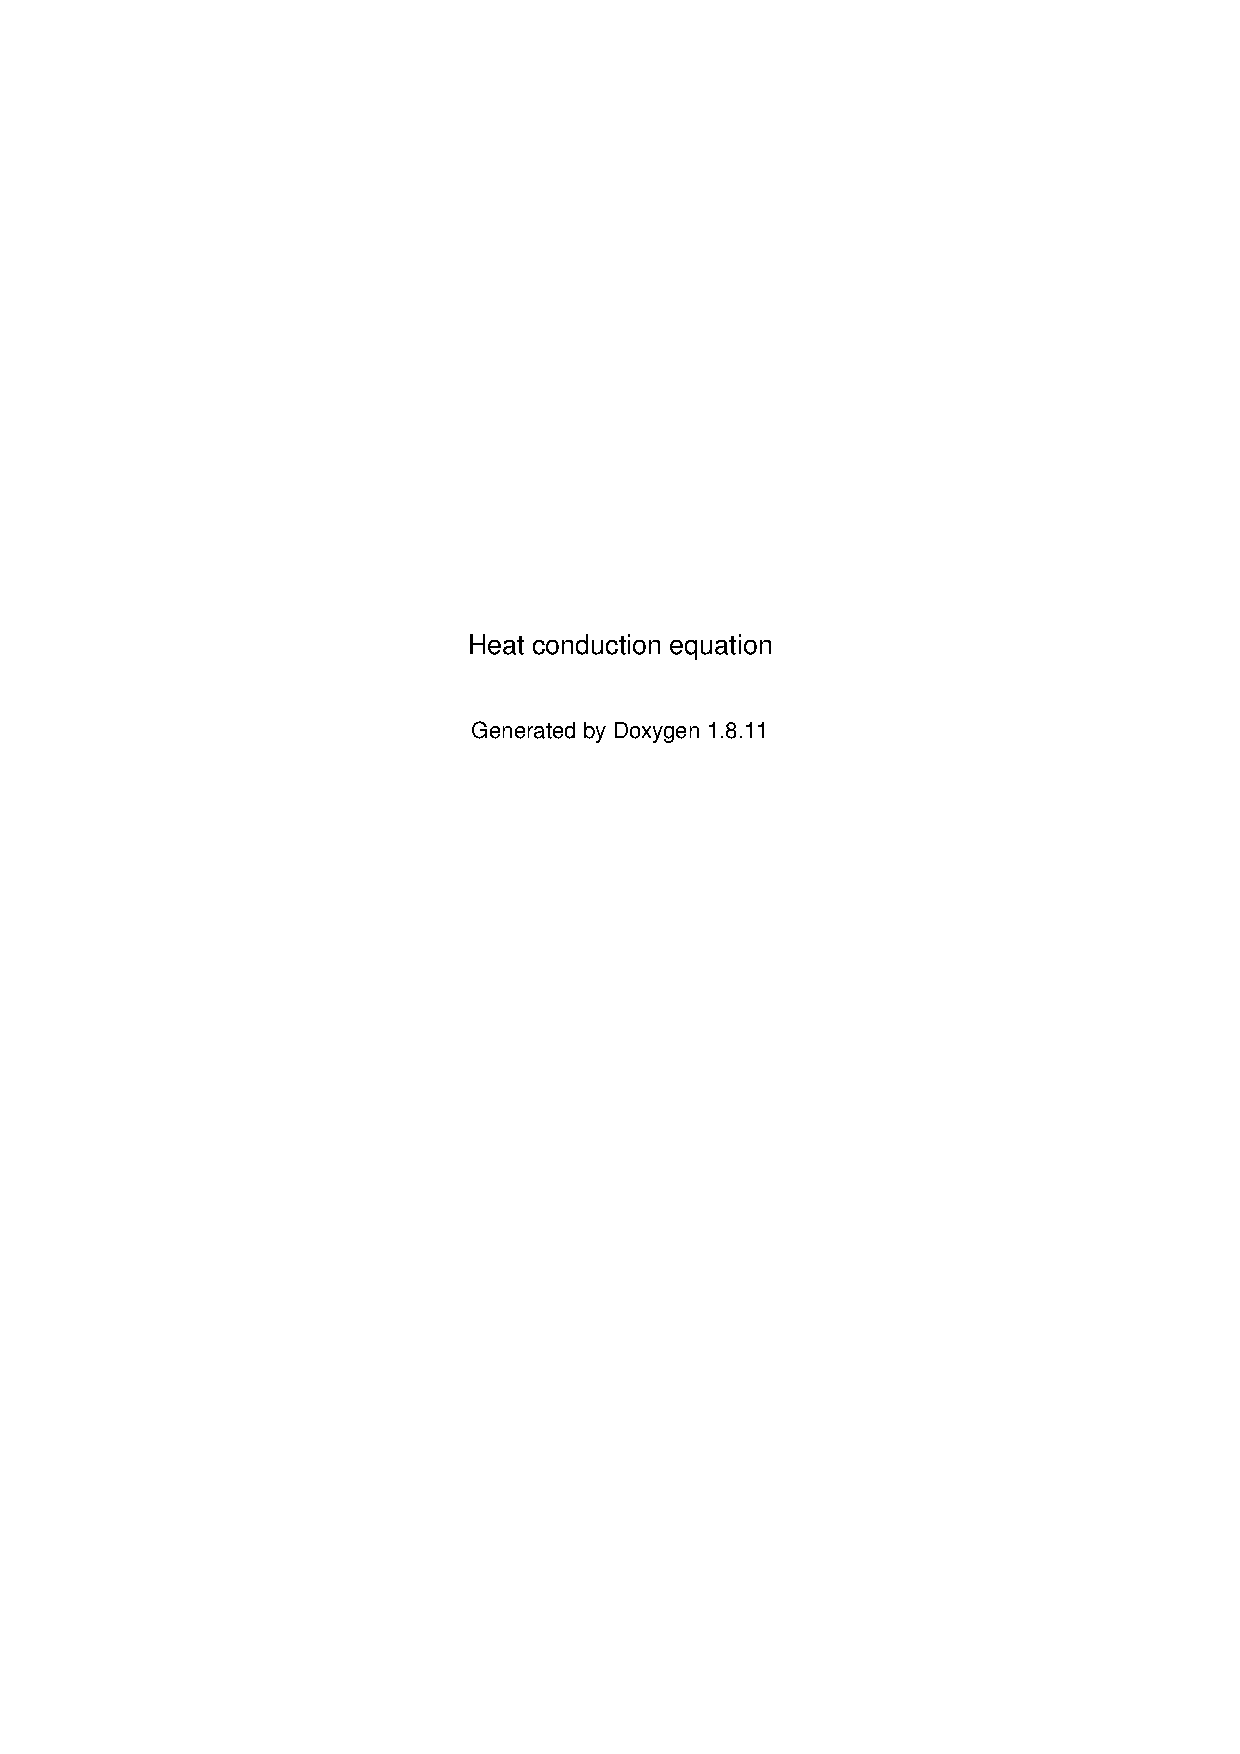
\includepdf[pages=-]{refman}

\end{document}

